\section{Challenges derived from including mobile devices}\label{challenges_derived_from_mobile_devides}
While the intrinsic challenges described in \textit{section \ref{intrinsic_challenges_of_grid_computing}} remain still valid, the inclusion of mobile devices in the Grid arises new issues that have to be taken into consideration while designing the system. Some challenges have been resolved by the evolution of technology and the new behaviors adopted by mobile users (\textit{section \ref{previous_works_and_limitations}}) but other ones still need to be dealt with.

\subsection{Network instability}
Compared to a computer, \textbf{a mobile device is afflicted by network instability more often}. This issue is linked to the \textbf{mobility factor} \cite{integrating_mobile_devices_into_grid} that comes with such devices, creating a \textbf{more dynamic and less reliable environment connection-wise}.

Aside from Wi-Fi connection (that still can suffer from instability but is generally stabler), the \textbf{main source of instability} comes from \textbf{mobile data connection}.
Enormous progress in mobile data connection technologies has been made, but still the reliability suffers, especially in use cases where having a stable connection is required. Recently, \textbf{5G technology is slowly emerging as the new technological leap}. But, as other works have observed \cite{5g_performances}, 5G is still in its infancy and, while offering \textbf{great performances under optimal condition}, it is affected by \textbf{greater instability compared to 4G}.

While discussing properties about mobile data technology, it is important to first understand the concept of handoff:
\begin{itemize}
    \item \textbf{Horizontal handoff}: occurs when the connection switches from one repeater to another. In the case of 5G this happens more often, since the technology requires a greater number of repeaters in order to work because of the different wave lengths used.
    \item \textbf{Vertical handoff}: occurs when the networking technology changes. This is still particularly a problem for 5G connections since, being less stable, they often require a switch to 4G ones.  
\end{itemize}
\begin{figure}[H]
    \centering
    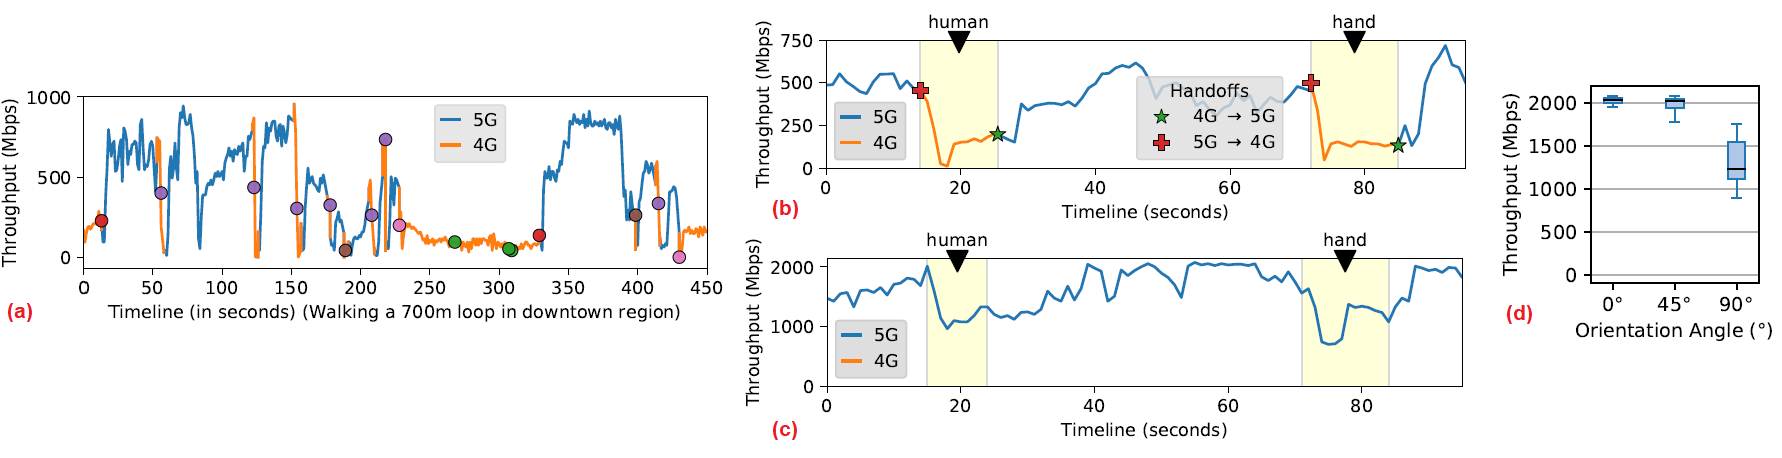
\includegraphics[width=\linewidth]{document/chapters/chapter_3/images/5G_performances.png}
    \caption{5G's throughput under different circumstances \cite{5g_performances}}
    \label{fig:5G_performances_graphs}
\end{figure}

Here are a few more relevant factors affecting the quality and performance of a mobile network:
\begin{itemize}
    \item \textbf{Traveling speed}\\
    Moving through space causes fluctuation in the stability of the connection, with usually better performances while standing still, a slight worsening while moving at walking pace and, finally, a progressive drop in performance with higher speeds. \textit{Figure \ref{fig:5G_performances_graphs} (a)} shows how a 5G network throughput varies over time by simply walking for 700 meters; in this graph, dots represent horizontal and/or vertical handoffs, showing how unstable mobile connections (especially 5G ones) are.
    \item \textbf{Obstacles}\\
    Having obstacles between the device and the connection source significantly alters performances. In simple terms, 4G utilizes signal waves in a more sparse way; on the other hand, 5G utilizes waves that are highly focused, requiring a trajectory to reach the device, whether being on LoS (line-of-sight, i.e. there are no obstacles between the device and the repeater) or on NLoS (non-line-of-sight, i.e. the repeater finds an indirect trajectory that bounces the signal using objects). \textit{Figure \ref{fig:5G_performances_graphs} (b)} shows how throughput varies in response of physical obstacles (a human body and a hand) when there are no efficient trajectories to reach the device; on the other hand, \textit{figure \ref{fig:5G_performances_graphs} (c)} shows the same phenomenon when there are many optimal trajectories for the signal waves.
    \item \textbf{Placement relative to the connection source}\\
    Even the way that the device is placed in space relatively to the connection source alters performances; generally speaking, this is due to the placement of the mobile device's antenna but, in the 5G case, it also depends on the orientation angle relatively to the source (\textit{figure \ref{fig:5G_performances_graphs} (d)}).
    \item \textbf{Weather}\\
    Also, atmospheric conditions slightly alter the efficiency of mobile connections, reaching up to 30\% reduction in throughput speed during rainfall on a 5G mobile network \cite{5g_performances}.
\end{itemize}

Since it will become the standard technology in the following years, a lot of examples using 5G have been used  but, even if with different severity, the same instability issues also apply to the other mobile data connection technologies. Three approaches (in ascending order of complexity) can be used to deal with the mobile devices network instability:
\begin{itemize}
    \item \textbf{Allowing contributing to the Grid only while using a Wi-Fi connection}.
    \item \textbf{Limiting contribution while on mobile data connection only to a few specific use cases} that do not require stability.
    \item \textbf{Implementing smart context-aware mechanisms} that take the decision to allow or not mobile data contribution based on a combination of technology type, throughput, movement in space (using accelerometers) and possibly current weather condition (using GPS).
\end{itemize}

Considering that, currently, \textbf{mobile connectivity data plans still have limited (although increasing) traffic available each month}, not all users may want to dedicate it to the Grid contribution; hence, \textbf{the second approach is probably the best one}, since it expands use cases and capabilities while not wasting effort on a slightly useful feature. Finally, active contribution to the Grid using mobile data increases battery consumption, which will now be discussed in the following section.

\subsection{Battery consumption}
Having devices that run on battery and are not connected to a reliable power source can be a source of problems for the Grid. \textbf{Sudden disconnections or failures have to be monitored anyway} since devices connected to a power source may be subjected to a sudden interruption of energy from the energy source or, more in general, it can incur in any kind of error. \textbf{The problem with mobile devices is more about the increased possibility of unplanned interruptions due to energy exhaustion of the battery}.
There are \textbf{five main factors} that \textbf{affect power usage} in mobile devices \cite{mobile_power_consumption}:
\begin{enumerate}
    \item \textbf{Hardware} (CPU, GPU, memory, storage, display, sensors);
    \item \textbf{Signaling and networking modules} (cellular network, Bluetooth, hotspot, Wi-Fi, GPS, FM radio);
    \item \textbf{Software} (operating system, background applications)
    \item \textbf{Usage patterns} (calling, internet browsing, social networks usage, gaming, music playback, video playback, running heavy applications);
    \item \textbf{Other factors} (inter-device communication, heating, aging and faulty battery).
\end{enumerate}
\textbf{How long the battery of a mobile device lasts depends on a combination of such factors}, ranging from days to (in extreme cases) only hours.

There are a set of \textbf{possible countermeasures} that limit the participation to the Grid only to devices that respect certain prerequisites that aim to mitigate this problem:
\begin{itemize}
    \item \textbf{External power source enforcement}\\
    The first obvious countermeasure is to only allow devices to contribute to the Grid while connected to a reliable power source. While certainly effective and totally feasible (since commonly mobile devices tend to be charged every day), this can limit the percentage of contributors active in a certain moment;
    \item \textbf{Battery health status check}\\
    Another method is checking for the device's battery health, allowing contribution to the Grid while disconnected from an external power source only to devices that have healthy battery units.
    \item \textbf{Battery percentage minimum level}\\
    The final countermeasure is allowing battery-powered contribution only when the device's battery is above a certain battery percentage.
\end{itemize}
The \textbf{best solution} to mitigate this problem is \textbf{a combination of the three countermeasures}, allowing healthy devices to contribute while above a certain battery percentage and limiting devices with an aged battery to only contribute while connected to a power source.

On a final note, what was discussed in this section can be mostly applied also to laptops, even though people usually tend to use them while connected to a power source.

\subsection{Even greater focus on security}
\textbf{As the number of smartphone increases}, the number of computers used by people are gradually declining (\textit{figure \ref{fig:global_sales_of_pcs_and_smartphones}}); as a direct consequence of this phenomenon, \textbf{malicious attack efforts are now being redirected to exploiting mobile devices' vulnerabilities}.
\begin{figure}[!ht]
    \centering
    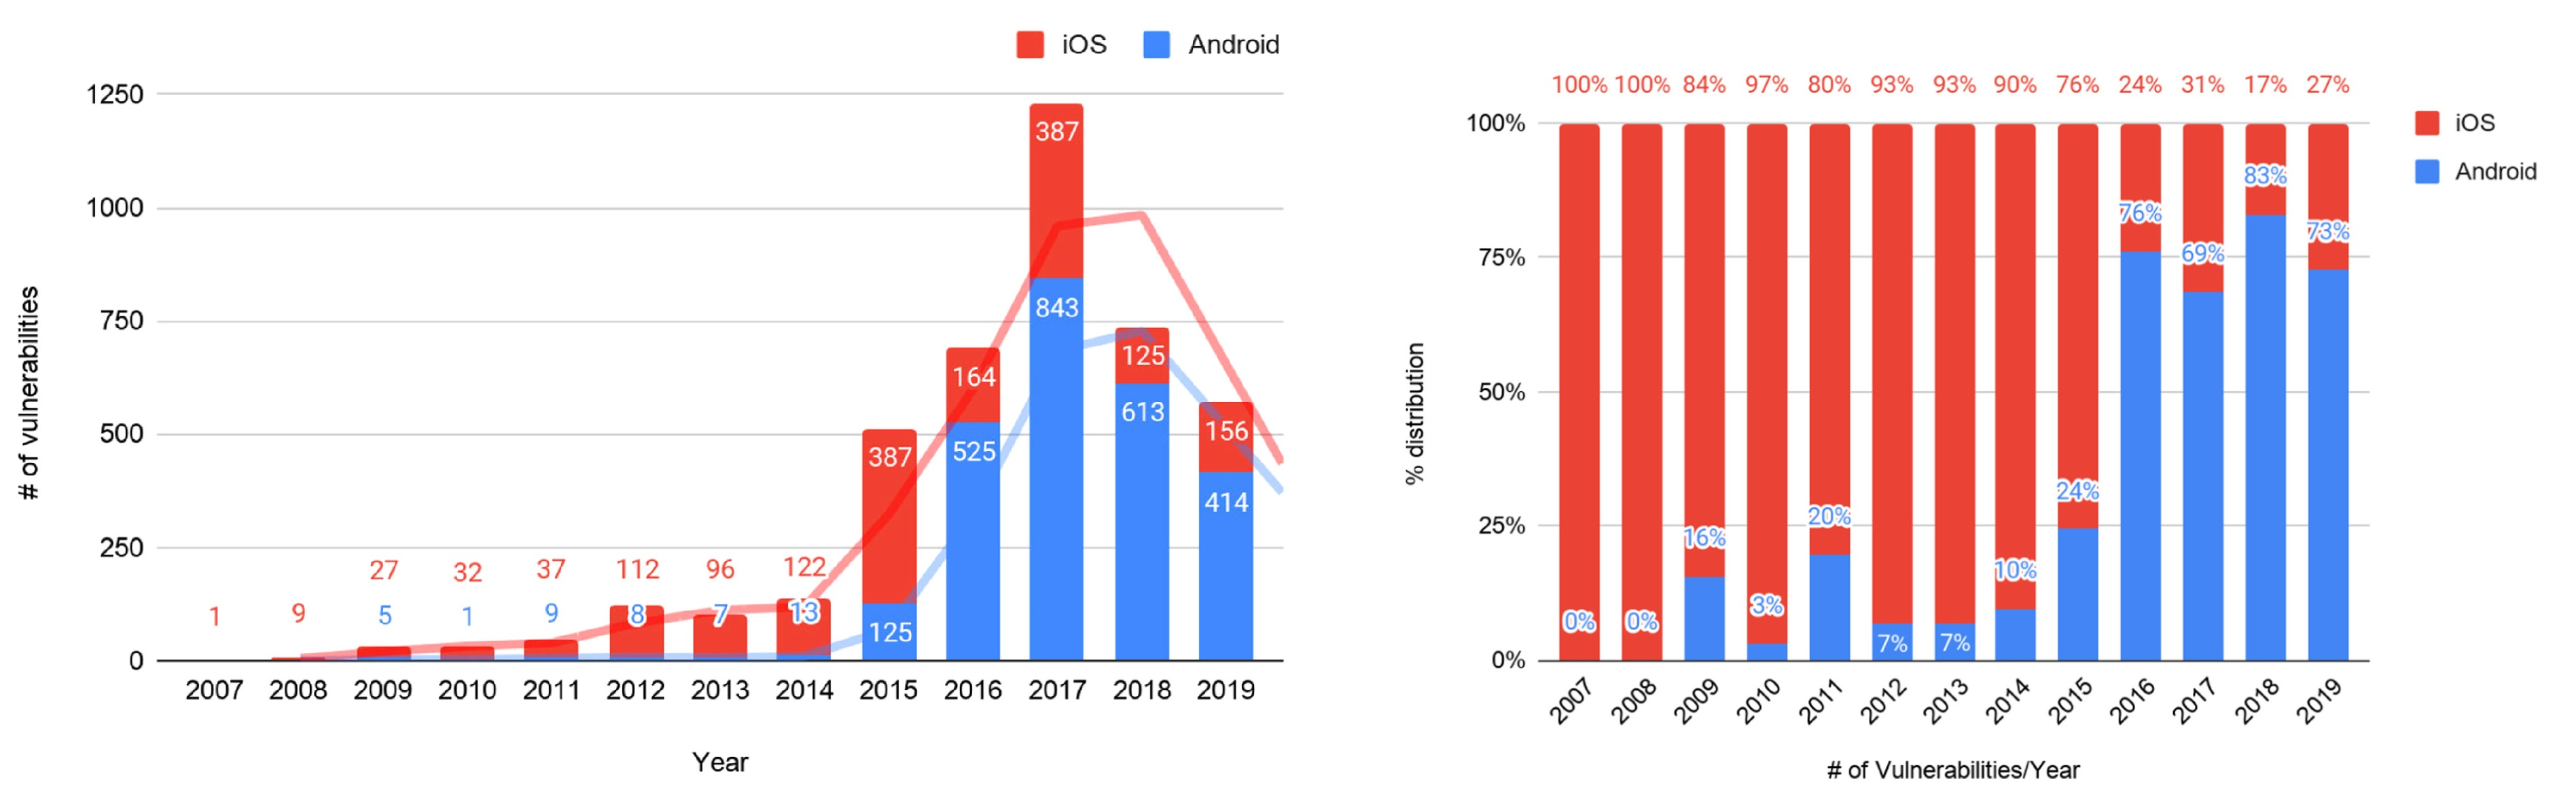
\includegraphics[width=\linewidth]{document/chapters/chapter_3/images/mobile_vulnerabilities.jpg}
    \caption{Number (left) and distribution (right) of known vulnerabilities on iOS and Android from 2007 to 2019 \cite{mobile_security}}
    \label{fig:mobile_vulnerabilities}
\end{figure}
\textit{Figure \ref{fig:mobile_vulnerabilities}} shows how \textbf{Android has more vulnerabilities compared to iOS}. This can be explained for the following two reasons:
\begin{itemize}
    \item \textbf{Android devices are more diffused}\\
    Attackers tend to attack these devices more, since the pool of individual units is larger (as shown in \textit{image \ref{fig:os_market_share_2012_to_2021}}) and thus, obtaining a profit is more likely.
    \item \textbf{iOS has more strict security measures} \cite{mobile_security}\\
    One of the byproducts of designing Android to be able to run a vast number of different hardware is the fact that compromises have to be made in order to grant compatibility. On the other hand, iOS runs on only a limited number of models, making it easier to design more effective security mechanisms. 
\end{itemize}
Through the \textbf{Linux Kernel}, Android resources are managed and protected. Furthermore, Android employs an \textbf{Application Sandbox} security mechanism, meaning that each application is run with a unique ID and the \textbf{processes are executed in spaces separated from each other and from the Kernel}, therefore preventing an application from interfering with the functioning of another. Despite this, Android employs an \textbf{authorization-based mechanism for accessing resources}; while \textbf{a process that has not the correct authorizations cannot access determinate resources}, the greatest weakness of this mechanism is the fact that \textbf{authorizations are granted by the user} who is not usually really aware of the implications of such choices. Application, consequently, can launch \textbf{various types of attacks depending on the type of authorizations} that they obtained. Another weakness of Android systems is the fact that \textbf{Application provenance is not guaranteed}; the Play Store's digital certificate can be easily obtained from malicious parties since Google only requires a fee paid by a credit card to get it (and payments might be done with a stolen credit card). Applications can also be installed from third parties, making it easier to introduce malicious software that is completely unchecked.

On the other hand, \textbf{iOS} utilizes a similar Sandbox system, but \textbf{authorizations are completely managed by the OS}, removing the possibility of human errors. From the Application provenance perspective, iOS' applications are only distributed by the App Store; developers have to register, pass a \textbf{vetting process} that evaluates the Application which, in case no harm is detected, is \textbf{digitally signed} and only then published on the store. This process makes more difficult the introduction of harmful applications.
\begin{figure}[H]
    \centering
    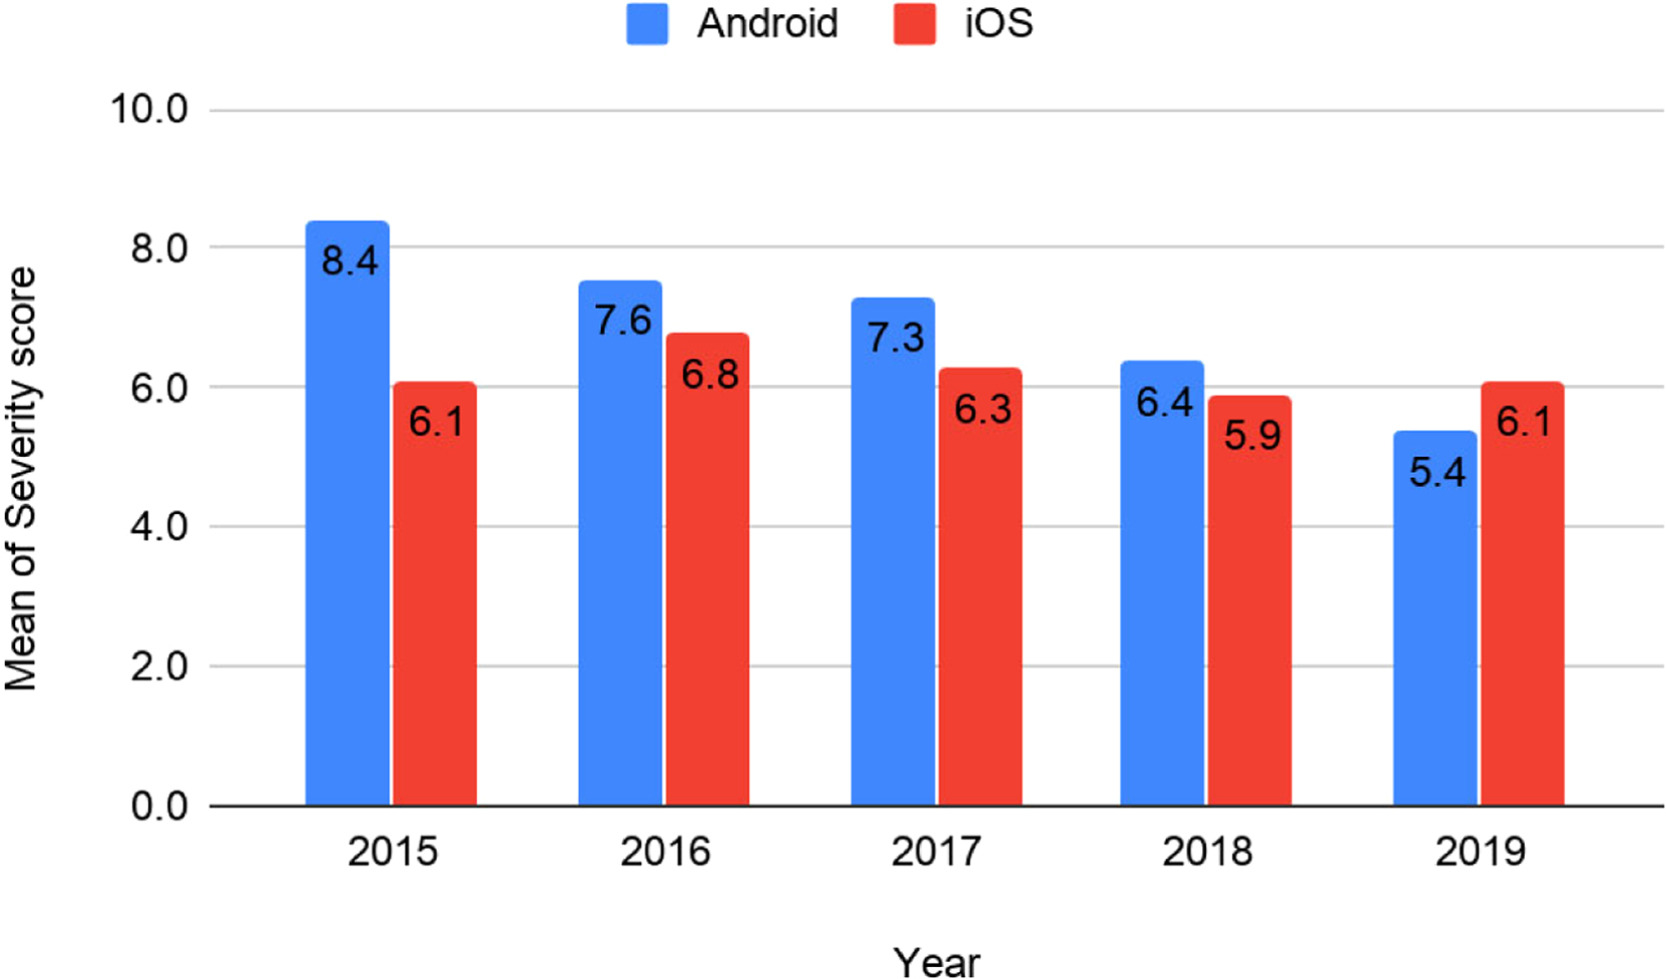
\includegraphics[scale=1.2]{document/chapters/chapter_3/images/mobile_vulnerabilities_severity.jpg}
    \caption{iOS and Android vulnerabilities severity score from 2015 to 2019 \cite{mobile_security}}
    \label{fig:mobile_vulnerabilities_severity}
\end{figure}
Even though iOS has the advantage when it comes to sheer number of security breaches, \textbf{with time the severity of Android's breaches has decreased, becoming less severe than the iOS' ones} (\textit{figure \ref{fig:mobile_vulnerabilities_severity}}).

This data highlights how it is particularly important to focus on the security of the Grid's Fabric Layer (\textit{section \ref{fig:fabric_layer}}) while dealing with mobile devices because, in the current panorama, they are the greatest source of security vulnerabilities, especially considering that the information inside them has great value for attackers.

\subsection{Compatibility issues}
\textbf{Developing software for mobile devices tends to be more prone to compatibility issues} compared to desktop environments, \textbf{due to the frequent changes that mobiles OSes undergo} in order to add new features, increase performances and enhance security. It is possible to distinguish between \textbf{two different types of compatibility} when it comes to software in relation to the version of the supporting SDK:

\begin{itemize}
    \item \textbf{Forward compatibility}, i.e. developing software that will run even on future OS distributions.
    \item \textbf{Backward compatibility}, i.e. developing software that runs also on older OS distributions.
\end{itemize}

\begin{figure}[!ht]
    \centering
    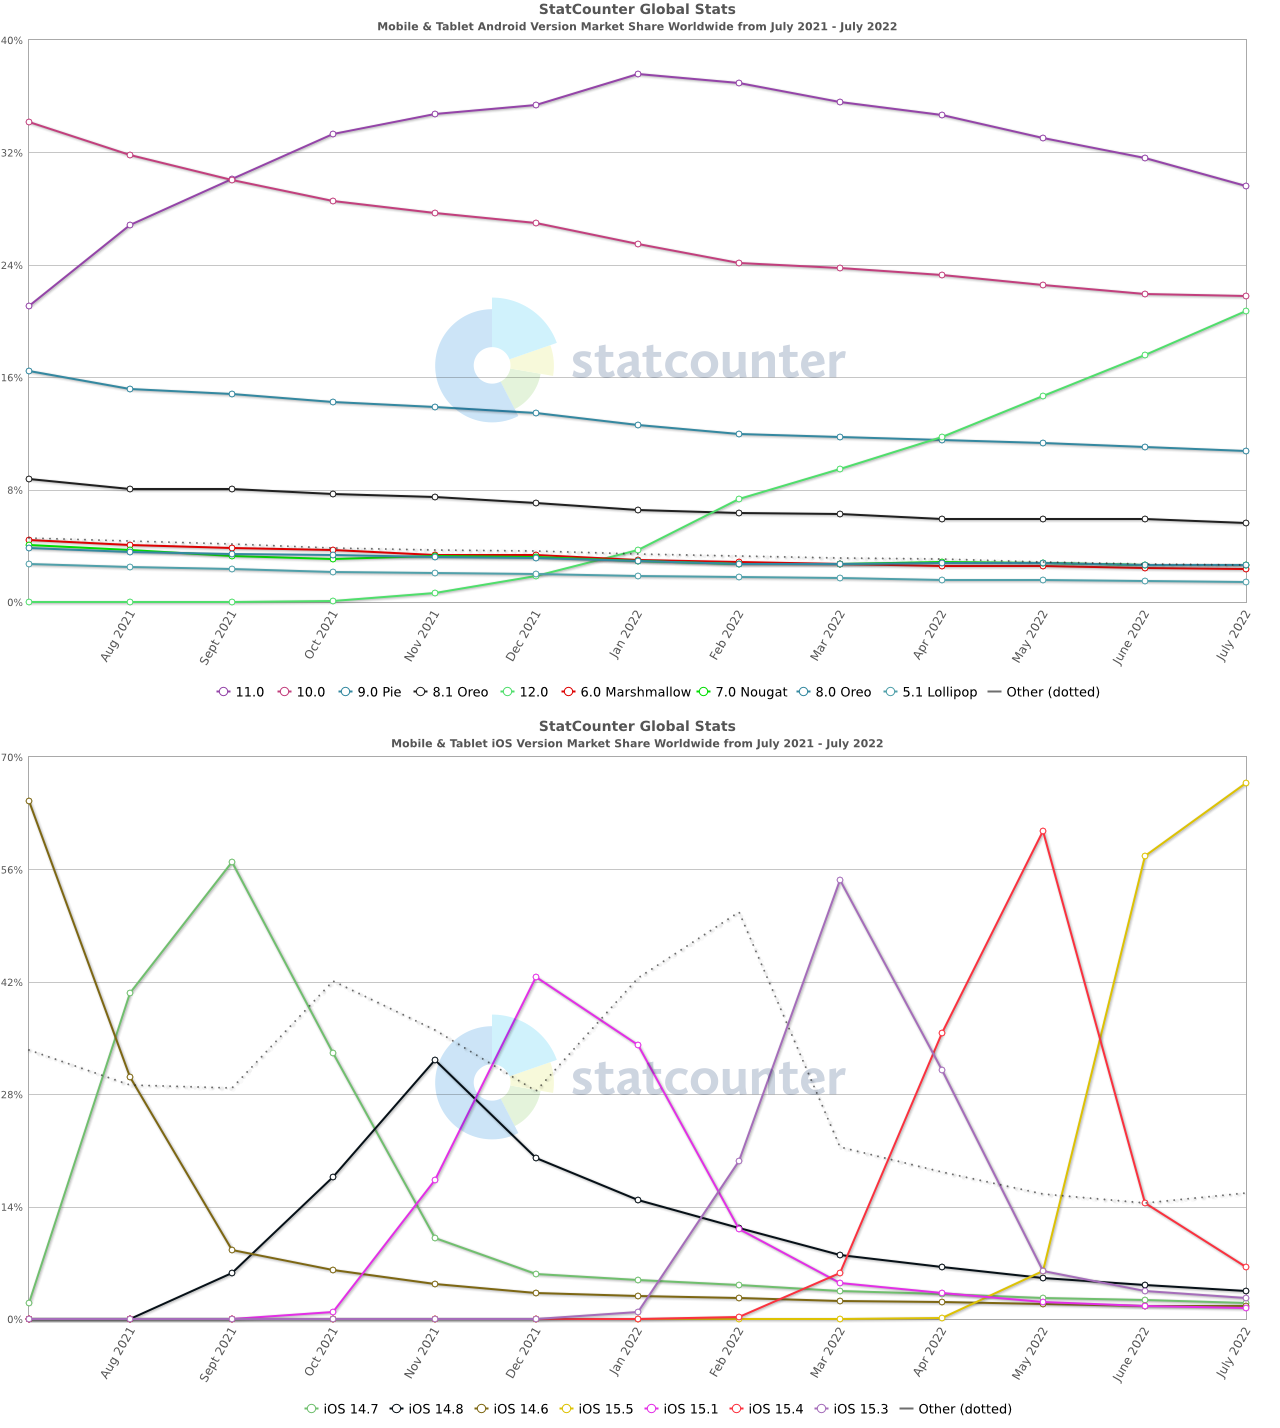
\includegraphics[scale=0.4]{document/chapters/chapter_3/images/stat_counter_ios_android.png}
    \caption{\href{https://gs.statcounter.com/}{Statcounter}'s statistics for OSes distribution between Android (top) and iOS (bottom) devices from July 2021 to July 2022}
    \label{fig:stat_counter_ios_android}
\end{figure}

Google's mobile OS uses an \textbf{API level system} in order to \textbf{check for the compatibility} of applications \textbf{across different versions of the OS} running on devices.
As the OS rapidly evolves, so \textbf{the APIs offered in the SDK frequently change}, \textbf{introducing compatibility problems}. Android documentation states that changes in API do not threaten forward compatibility, but this turns out not to really be the case:

\begin{quotation}
    \textit{"Even if Google claims that Android apps do not suffer from forward compatibility issues, mainly because removed APIs are still kept in the framework side as hidden APIs, forward compatibility induced APIs are still encouraged to be replaced because of security and performance concerns. Furthermore, since hidden APIs are also subject to remove or change, \textbf{forward compatibility is} also \textbf{not fully guaranteed in practice} anyway." \cite{automating_android_api_compatibility_issues}}
\end{quotation}

\textbf{Backward compatibility}, on the other hand, \textbf{tends not to be a great concern}, resulting only in incompatibility issues due to developers setting an improperly low \textbf{minSdkVersion} flag (in order to target as many devices as possible) without actually testing if the application works on older Android's releases.

\begin{quotation}
    \textit{"Accessing backward compatibility induced APIs, without proper protection, will simply result in app crashes, giving poor experience to end-user." \cite{automating_android_api_compatibility_issues}}
\end{quotation}

Similarly, \textbf{APIs in iOS' SDK have compatibility issues between different versions of the OS}; Since changes are generally less drastic, it is \textbf{easier to test} for compatibility issues (given also the limited number of different Apple devices), but, on the other hand, iOS development suffers from a great limitation: \textbf{development of native apps can only be done on Apple's line of computers}.

Whether the development for Android and iOS devices uses native technologies or cross-platform technologies (such as React Native), \textbf{there is really no solution to this compatibility issue other than extensive testing} for every targeted version of both OSes, making the \textbf{development on such platforms more time-consuming and complex} both at the beginning and in the maintenance life cycle.
